\documentclass[pageno]{jpaper}

\def\BibTeX{{\rm B\kern-.05em{\sc i\kern-.025em b}\kern-.08em
    T\kern-.1667em\lower.7ex\hbox{E}\kern-.125emX}}

% Ensure letter paper
\pdfpagewidth=8.5in
\pdfpageheight=11in

\newcommand{\todo}[1]{{{\color{red} [TODO: #1]}}}
\newcommand{\TODO}[1]{{{\color{red} [TODO: #1]}}}
\newcommand{\tianyin}[1]{{{\color{red} [ty: #1]}}}
\newcommand{\tyler}[1]{{{\color{red} [tyler: #1]}}}
\newcommand{\edit}[1]{{{\color{blue} [#1]}}}
\newcommand{\tofill}[1]{{{\color{red} #1}}}
\newcommand{\checked}[1]{{{#1}}}
\newcommand{\xudong}[1]{{\color{red} [xd: #1]}}
\newcommand{\Space}[1]{}
\newcommand{\Fix}[1]{{\color{red}#1}}

\usepackage{listings}
\usepackage{color}
\usepackage{multirow}
\usepackage{booktabs}
\usepackage{amssymb}
\usepackage[T1]{fontenc}
\usepackage{inconsolata}
\usepackage{xcolor}
\usepackage{colortbl}
\usepackage{xspace}
% \usepackage[inline]{enumitem}

%\newcommand{\comment}[1]{{}}

\usepackage{tikz}
\newcommand*\BC[1]{%
	\begin{tikzpicture}[baseline=(C.base)]
		\node[draw,circle,fill=black,inner sep=0.1pt](C) {\textcolor{white}{#1}};
	\end{tikzpicture}}
	%\end{tikzpicture}\hspace{2px}}

\definecolor{gray}{gray}{0.5}
\definecolor{LightGray}{gray}{0.85}
\definecolor{VeryLightGray}{gray}{0.90}
\definecolor{ForestGreen}{rgb}{0.13, 0.55, 0.13}
\definecolor{Maroon}{rgb}{0.5, 0.0, 0.0}
\definecolor{darkpastelred}{rgb}{0.76, 0.23, 0.13}

\newcommand{\acto}{Acto\xspace}
\newcommand{\actoblack}{Acto-$\blacksquare$\xspace}
\newcommand{\actowhite}{Acto-$\square$\xspace}
\newcommand{\spec}{test plan}

\newcommand{\dirtystate}{dirty-state}
\newcommand{\stalestate}{stale-state}
\newcommand{\volatilestate}{volatile-state}
\newcommand{\dirtystatecap}{Dirty-state}
\newcommand{\stalestatecap}{Stale-state}
\newcommand{\volatilestatecap}{Volatile-state}

\newcommand{\operator}{operator\xspace}
\newcommand{\operatorcap}{Operator\xspace}
\newcommand{\operators}{operators\xspace}
\newcommand{\operatorscap}{Operators\xspace}
\newcommand{\canonicalizes}{normalizes\xspace}
\newcommand{\canonicalization}{normalization\xspace}

\newcommand{\opcap}{Controller}
\newcommand{\opscap}{Controllers}
\newcommand{\op}{controller}
\newcommand{\ops}{controllers}

\newcommand{\para}[1]{\smallskip\noindent {\bf #1} }
\newcommand{\tworow}[1]{\multirow{2}{*}{#1}}

\newcommand{\caop}{Cass-op\xspace}
\newcommand{\crdbop}{Cockroach-op\xspace}
\newcommand{\knop}{KnativeOp\xspace}
\newcommand{\mgopone}{Mongodb-op-2\xspace}
\newcommand{\mgoptwo}{MongodbOp\xspace}
\newcommand{\xtop}{Xtradb-op\xspace}
\newcommand{\rbop}{RabbitmqOp\xspace}
\newcommand{\rdopone}{spothome/Redis-op\xspace}
\newcommand{\rdoptwo}{OKT/Redis-op\xspace}
\newcommand{\tiop}{Tidb-op\xspace}
\newcommand{\zkop}{ZookeeperOp\xspace}

\newcommand{\object}{state object}
\newcommand{\objectcap}{State object}
\newcommand{\objects}{state objects}
\newcommand{\objectscap}{State objects}


\newcommand*\circled[1]{\tikz[baseline=(char.base)]{
    \node[shape=circle,draw,inner sep=0.5pt] (char) {#1};}}

\newcommand*\circledblack[1]{\tikz[baseline=(char.base)]{
            \node[fill=black,shape=circle,draw,inner sep=0.5pt] (char) {\color{white}#1};}}

\newenvironment{packed_itemize}{
\begin{list}{\labelitemi}{\leftmargin=1.0em}
 \setlength{\itemsep}{2.5pt}
 \setlength{\parskip}{0pt}
 \setlength{\parsep}{0pt}
 \setlength{\headsep}{0pt}
 \setlength{\topskip}{0pt}
 \setlength{\topmargin}{0pt}
 \setlength{\topsep}{0pt}
 \setlength{\partopsep}{0pt}
}{\end{list}}

\newenvironment{packed_enumerate}{
\vspace{-1.8ex}
\begin{enumerate}[label=(\arabic*),leftmargin=1.7em]
 \setlength{\itemsep}{1.5pt}
 \setlength{\parskip}{0pt}
 \setlength{\parsep}{0pt}
 \setlength{\headsep}{0pt}
 \setlength{\topskip}{0pt}
 \setlength{\topmargin}{0pt}
 \setlength{\topsep}{0pt}
 \setlength{\partopsep}{0pt}
}{\end{enumerate}
\vspace{-1.8ex}
}

% \lstset{language=Go,
%   basicstyle=\ttfamily\scriptsize,
%   keywordstyle=\color{blue}\ttfamily,
%   stringstyle=\color{red}\ttfamily,
%   commentstyle=\color{green}\ttfamily
% }

\colorlet{punct}{red!60!black}
\definecolor{background}{HTML}{EEEEEE}
\definecolor{delim}{RGB}{20,105,176}
\colorlet{numb}{magenta!60!black}

\lstdefinelanguage{json}{
    basicstyle=\footnotesize\ttfamily,
    numbers=left,
    numberstyle=\footnotesize,
    stepnumber=1,
    numbersep=8pt,
    showstringspaces=false,
    breaklines=true,
    frame=lines,
    backgroundcolor=\color{background},
    literate=
     *{0}{{{\color{numb}0}}}{1}
      {1}{{{\color{numb}1}}}{1}
      {2}{{{\color{numb}2}}}{1}
      {3}{{{\color{numb}3}}}{1}
      {4}{{{\color{numb}4}}}{1}
      {5}{{{\color{numb}5}}}{1}
      {6}{{{\color{numb}6}}}{1}
      {7}{{{\color{numb}7}}}{1}
      {8}{{{\color{numb}8}}}{1}
      {9}{{{\color{numb}9}}}{1}
      {:}{{{\color{punct}{:}}}}{1}
      {,}{{{\color{punct}{,}}}}{1}
      {\{}{{{\color{delim}{\{}}}}{1}
      {\}}{{{\color{delim}{\}}}}}{1}
      {[}{{{\color{delim}{[}}}}{1}
      {]}{{{\color{delim}{]}}}}{1},
}

\lstdefinelanguage{godep}{
  % Keywords as defined in the language grammar
  morekeywords=[1]{%
    cr,Spec,Backup,Enabled,Sharding},
  % Built-in functions
  keywordstyle=[4]\color{blue},
  morekeywords=[2]{%
    append,cap,close,complex,copy,delete,imag,%
    len,make,new,panic,print,println,real,recover},
  % Pre-declared types
  morekeywords=[3]{%
    bool,byte,complex64,complex128,error,float32,float64,%
    int,int8,int16,int32,int64,rune,string,%
    uint,uint8,uint16,uint32,uint64,uintptr},
  % Constants and zero value
  morekeywords=[4]{return},
  % Strings : "foo", 'bar', `baz`
  morestring=[b]{'},
  morestring=[b]{`},
  % Comments : /* comment */ and // comment
  comment=[l]{//},
  morecomment=[s]{/*}{*/},
  % Options
  sensitive=true,
  tabsize=2,
  numbers=none,
  frame=no,
  basicstyle=\scriptsize\ttfamily,
%  basicstyle=\footnotesize\ttfamily,
  keywordstyle=\color{darkpastelred}\ttfamily\bfseries,
  commentstyle=\color{ForestGreen},
%  numbers=left,
%  numbersep=5pt,
  showstringspaces=false,
  stringstyle=\color{blue},
}

\lstdefinelanguage{myGo}{
  % Keywords as defined in the language grammar
  morekeywords=[1]{%
    break,default,func,interface,select,case,defer,go,map,%
    struct,chan,else,goto,package,switch,const,fallthrough,%
    if,range,type, continue,for,import,return,var},
  % Built-in functions
  morekeywords=[2]{%
    append,cap,close,complex,copy,delete,imag,%
    len,make,new,panic,print,println,real,recover},
  % Pre-declared types
  morekeywords=[3]{%
    bool,byte,complex64,complex128,error,float32,float64,%
    int,int8,int16,int32,int64,rune,string,%
    uint,uint8,uint16,uint32,uint64,uintptr},
  % Constants and zero value
  morekeywords=[4]{true,false,iota,nil},
  % Strings : "foo", 'bar', `baz`
  morestring=[b]{"},
  morestring=[b]{'},
  morestring=[b]{`},
  % Comments : /* comment */ and // comment
  comment=[l]{//},
  morecomment=[s]{/*}{*/},
  % Options
  sensitive=true,
  tabsize=2,
  numbers=none,
  frame=no,
  basicstyle=\scriptsize\ttfamily,
%  basicstyle=\footnotesize\ttfamily,
  keywordstyle=\color{darkpastelred}\ttfamily\bfseries,
  commentstyle=\color{ForestGreen},
%  numbers=left,
%  numbersep=5pt,
  showstringspaces=false,
  stringstyle=\color{blue},
}

% \lstset{ % add your own preferences
%     frame=single,
%     basicstyle=\footnotesize,
%     keywordstyle=\color{red},
%     numbers=left,
%     numbersep=5pt,
%     showstringspaces=false,
%     stringstyle=\color{blue},
%     tabsize=2,
%     language=myGo % this is it !
% }

% \newcommand\YAMLcolonstyle{\color{red}\mdseries}
% \newcommand\YAMLkeystyle{\color{black}\bfseries}
% \newcommand\YAMLvaluestyle{\color{blue}\mdseries}

\definecolor{cornellred}{rgb}{0.7, 0.11, 0.11}
\definecolor{cadetgrey}{rgb}{0.57, 0.64, 0.69}
\definecolor{battleshipgrey}{rgb}{0.52, 0.52, 0.51}
\newcommand\YAMLcolonstyle{\color{black}}
\newcommand\YAMLkeystyle{\color{cornellred}}
\newcommand\YAMLvaluestyle{\color{blue}}
\lstdefinelanguage{myyaml}
{
  keywords={true,false,null,y,n},
  keywordstyle=\color{darkgray}\bfseries,
  basicstyle=\YAMLkeystyle\footnotesize\ttfamily,   % assuming a key comes first
  sensitive=false,
  comment=[l]{\#},
  morecomment=[s]{/*}{*/},
  % basicstyle=\footnotesize\ttfamily,
  commentstyle=\color{battleshipgrey}\ttfamily,
  stringstyle=\YAMLvaluestyle\ttfamily,
  moredelim=[l][\color{orange}]{\&},
  moredelim=[l][\color{magenta}]{*},
  moredelim=**[il][\YAMLcolonstyle{:}\YAMLvaluestyle]{:},   % switch to value style at :
  morestring=[b]',
  morestring=[b]",
  literate =    {>}{{\textcolor{red}\textgreater}}1
                {|}{{\textcolor{red}\textbar}}1
                {\ -\ }{{\mdseries\ -\ }}3,
}


\definecolor{ballblue}{rgb}{0.13, 0.67, 0.8}
\definecolor{bondiblue}{rgb}{0.0, 0.58, 0.71}
\definecolor{cobalt}{rgb}{0.0, 0.28, 0.67}
\definecolor{copper}{rgb}{0.72, 0.45, 0.2}
\definecolor{darkblue}{rgb}{0.0, 0.0, 0.55}

% Comments
\newcommand\lalith[1]{{\color{purple}{Lalith:#1}}}

\newcommand{\dummy}{DUMMY}
\definecolor{light-gray}{gray}{0.95}
\newcommand{\code}[1]{\texttt{#1}}

\newcommand{\newbugs}{59 }
\newcommand{\confirmedbugs}{47 }
\newcommand{\fixedbugs}{31 }
\newcommand{\fprate}{12.77\% }

\lstset{
  basicstyle=\tiny,
  columns=fullflexible,
  frame=single,
  breaklines=true,
  numbers=left,
}


\begin{document}

\date{}

% make title bold and 14 pt font (Latex default is non-bold, 16 pt)
\title{Research Proposal}
\author{Muhammad Taha}

\maketitle

\section{Introduction}
    Federated Learning involves training a shared global model using local data and compute on various user devices.
    Several approaches have been proposed to implement this paradigm starting with Federated Averaging~\cite{DBLP:journals/corr/McMahanMRA16}.
    However, not many of these approaches consider low-end devices that are unable to perform training. 
    This has implications for fairness due to introduction of systematic bias, in addition to degradation in model accuracy.
    Recent works such as FedProx (2) and Hassas (3) have attempted to include slow devices by incorporating partial work and serving a subset model according to device characteristics, respectively. 
    These approaches have been evaluated on large-scale simulations using LEAF Benchmark~\cite{DBLP:journals/corr/abs-1812-01097} and a small-scale testbed of mobile devices in case of Hassas.
    To the best of our knowledge, none of these works have been evaluated on mid-scale federated learning systems using actual mobile devices with a sufficiently large number of clients.
    \newline
    Significance of the problem stems from the need to include low-end smart phones and IOT devices in the process of training the data. Inclusitivity of such users will allow for a  more precise model to be generated as the training data will be diverse and more  reflective of real life. Moreover, in the developing countries where more than 57\% of population are categorised as low-end users, their exclusion in the past models~\cite{10.1145/3446382.3448652} will lead to great inaccuracies and biasness. The approach of having sub-models in these devices will increase the likelihood for to train models even in the  case of limited poor connectivity and limited bandwidth. Overall, the concept of Hasaas will create a better privacy preserving and resource efficient model.
\section{Related Work}
    \textbf{HeteroFL} challenges the assumption that local models must have the same architecture as the global model.~\cite{DBLP:journals/corr/abs-2010-01264} On the other hand, \textbf{FedDST} proposes approaches to make on-device computation and in-network communication more efficient.~\cite{DBLP:journals/corr/abs-2112-09824} \textbf{FedProx} incorporates partial work to include low-end devices~\cite{DBLP:journals/corr/abs-1812-06127}. However, these frameworks mostly leverage the \textbf{LEAF} benchmark for experimentation.~\cite{DBLP:journals/corr/abs-1812-01097} In addition,~\cite{232971} aims to demonstrate the impact of straggler devices by measuring the impact of cpu resource heterogeneity on training time. The evaluation is conducted using an emulated environment with clients running in Docker containers deployed on a AWS EC2 Virtual Machine instance. The following FL approches perform evaluations using small-scale testbeds of real-world devices. \textbf{PruneFL} uses a set of Raspberry Pi devices connected to a central server (PC) and a simulated setting.~\cite{DBLP:journals/corr/abs-1909-12326} Time measurements from Raspberry Pi devices are used for experiments conducted on the simulated setting. \textbf{Hermes} leverages structured pruning to find a small subnetwork for each device and aggregating across overlapping parameters to learn a structured sparse deep neural network.~\cite{10.1145/3447993.3483278} The framework is evaluated on a testbed of 3 Google Pixel smartphones connected to a central server. Similarly,~\cite{9139810} utilized a testbed of 4 devices with different device characteristics to to evaluate their approach using the MNIST dataset. Hence, we find few works that have performed evaluations on real-world devices.

% reference deployed FL applications
% papers evaluated on testbed of real devices
\graphicspath{ {./images/} }

\section{What approaches did we try?}
    Intially, we started with comparing the testbed framework with flower by training
    on each framework with 4 devices. This was done to conduct a cost-benefit analysis
    of each framework so that we can make an informed decision keeping in mind our goals
    which include scalability and support to ensure a robust and efficient implementation of our system. Flower is an open-source framework which provides intuitive APIs and an interface to implement custom strategies. However, support for android training in Java and Kotlin is still under development, which is why we implemented our own android application for training purposes. \\

    \begin{table}[h]
    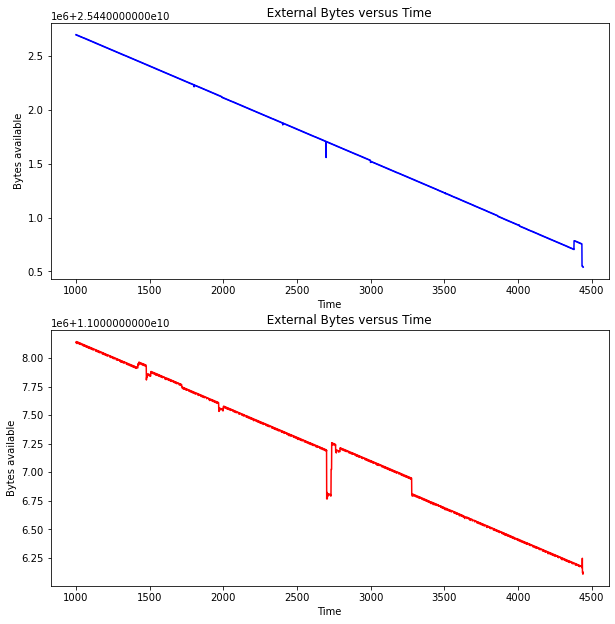
\includegraphics[scale=0.38]{extbytesvstime}
    \caption{External Bytes Available: As shown in Figure 1, since we are logging data every second, this is why the external storage bytes are constantly decreasing.}
    \end{table}
    
    Our existing implementation in testbed for device information logging requires root access. Since this is not conducive for the remote, continuous infrastructure that we want to deploy, we integrated support for memory profiling, cpu profiling, among other characteristics that do not require root access, using the android Activity Manager API.
    Due to the remote nature of the deployment, the FL task should be independent of the need for user interference. Specifically, we eliminated the need for manual loading of data from the server and beginning FL task execution. \\

    Keeping in mind android system optimizations, it was important to ensure that our application ran in the foreground so that it is given higher priority and is less likely to be killed in high memory pressure situations. We also anticipated reduced application performance when the system limited its resources like CPU and Memory usage, for example, to conserve battery life. If the application is killed by the Operating System, it will lose its connection to the server, resulting in lost updates and incur an additional overhead of data reloading. This can be a significant issue, particularly in our case, where we expect large number of clients and longer training times. \\

    \begin{table}[h]
    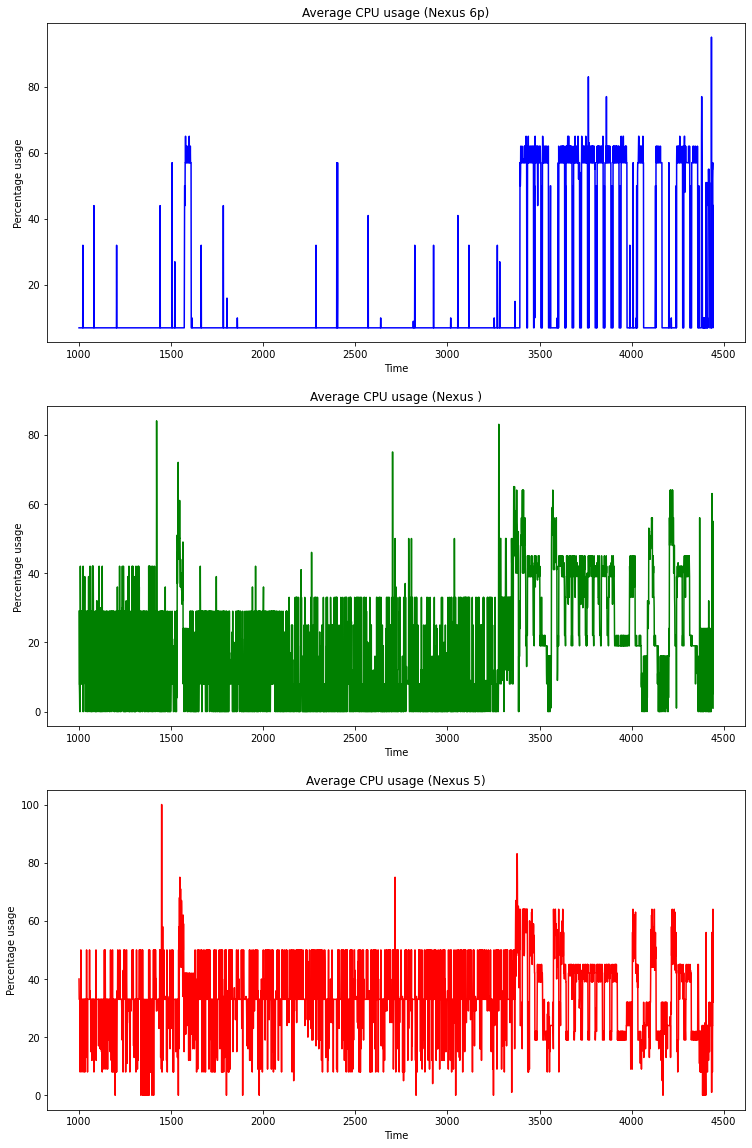
\includegraphics[scale=0.30]{cpuprof}
    \caption{CPU Profile: In the first round, the training completes for each device for the set number of epochs. However, due to a systematic error, the client thread blocks and the server waits for the client parameters so no CPU is utilized for the FL task. When one of the devices was switched to the foreground, the blockage is removed and the task resumes. This is a bug in our system which we are working on fixing.}
    \end{table}

    Due to time constraints, the intial idea of developing an application that would generate real-world data by providing users with an attractive incentive, was postponed. As a result, we decided to use an emulated dataset and partitioning the data among the users. From an implementation perspective, the dataset will be hosted on a centralized server. Clients connecting to the server will be assigned respective client IDs which will be used by the clients to fetch their respective data partitions from the central server. Due to similar reasons as above, the implementation of Hassas was also postponed. Instead, we are conducting evaluations using the Federated Averaging algorithm. \\

    In order to access the performance and impact of Flower on low end phones, we mainly aimed at creating a sufficient user pool of mainly android phones with 2 to 3 GB RAM. We are approaching the LUMS student body, PDC staff, and MBM workers. However, we have found most devices to be mostly 4GB and above. Hence, we explored options outside LUMS in our individual capacity. As a result of our efforts, we were able to gather around 10 devices (< 4GB RAM) and 5 devices (> 3GB RAM). We expect to gather a much larger number of fast devices, but intend to maintain an appropriate ratio between the two. We are also reaching out to mobile phone vendors who sell used phones. If we are able to reach some arrangement with them, we will be able to leverage many devices with diverse characteristics. \\

    \begin{table}[]
        \begin{tabular}{llll}
        \textbf{RAM (GB)}  & \textbf{Quantity} \\ 
        1                               & 1        \\
        2                               & 13        \\
        3                               & 8        \\
        4                               & 5        \\

        \end{tabular}
        \caption{Device Characteristics (By RAM)} 
    \end{table}

    (Metrics)
    cpu profile, memory profile, os interaction (timer interrupts, context switches), os heterogeneity (base profiling across devices)

    % \begin{table}[]
    %     \begin{tabular}{llll}
    %     \cline{1-1}
    %     \multicolumn{1}{|l|}{Model} & RAM(GB) & Quantity \\ \cline{1-1}
    %     Nexus 5X                    & 2       & 1        \\
    %     Nexus 6P                    & 3       & 2        \\
    %     Nexus 5                     & 2       & 4        \\
    %     Nexus 6                     & 3       & 3        \\
    %     Vivo Y12                    & 3       & 1        \\
    %     Oppo A37                    & 2       & 1        \\
    %     X                           & 2       & 1        \\
    %     Oppo A71K                   & 2       & 1        \\
    %     X                           & 2       & 1        \\
    %     Galaxy A21                  & 3       & 1        \\
    %     Techno Camon 18T            & 2       & 1        \\
    %     Galaxy S7 Edge              & 4       & 1        \\
    %     Infinix Smart 6             & 3       & 1        \\
    %     P8 Lite                     & 2       & 1        \\
    %     X                           & 2       & 1        \\
    %     X                           & 2       & 1        \\
    %     Galaxy S9 Plus              & 4       & 1        \\
    %     Galaxy S9                   & 4       & 1        \\
    %     Galaxy S8                   & 4       & 1        \\
    %     Galaxy S10                  & 4       & 1        \\
    %     Nokia 1                     & 1       & 1        \\
    %     \end{tabular}
    %     \caption{User Base Device Characteristics} 
    % \end{table}

    From our earlier experience of running FedAvg on Flower in a controlled setup, we postulate that the FL background process can be permanently interrupted at the client side due to mainly two reasons: the device is powered off, the process is killed by the system, or if it crashes due to some reason. Device state changes will be very frequent with real users. Hence, we are trying to add a restart mechanism which will essentially relaunch the process after device reboots and if the process is killed. To better analyse and inspect the reason for OS killing the App, we need to understand the OS interaction with App by performing crash analytics. Our crash analytics will include the context switching frequency, interupt frequency, and I/O Wait Time. Context switching frequency will tell us how difficult it is for the app to simultenously train data and log API metrics in the local storage. On the other hand, interupt frequency and I/O wait time will provide us with the insight of how much the App is competing for resources such as memory and CPU to carry out its tasks. \\

    \begin{table}[h]
        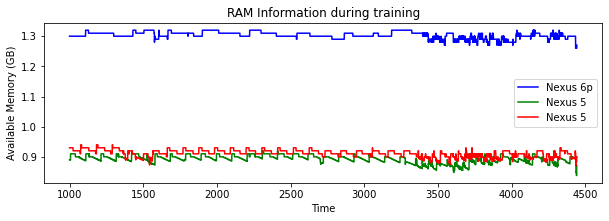
\includegraphics[scale=0.38]{freemem}
        \caption{Free Memory}
    \end{table}
    
    Once, we have sucessfully evaluated Federated Averaging process on the users, we aim to implement Hassas using the strategy interface in Flower.

% reference deployed FL applications
% papers evaluated on testbed of real devices
\begin{table}
    \footnotesize
    \centering
    \begin{tabular}{lccc}
        \textbf{Assignment} & \textbf{Deadline}  & \textbf{Members Responsible}\\
        
        Literature Review                       & Feb 17          & All                     \\
        Platform Evaluation                     & Feb 20          & Taha, Maaz            \\
        FL Deployment (4 Devices)      & Feb 26          & Hamza, Taha             \\
        FL Deployment (20 Devices)     & Mar 15          & Taha, Hamza             \\
        Mid Report                              & Mar 30          & All                     \\
        Application Prototype                   & April 1         & All, Shazer (Lead)            \\
        App Integration                             & April 5         & Shazer, Taha        \\
        Testing                                 & April 5         & Maaz, Hamza         \\
        User-base Development                   & April 15        & All                 \\
        Baseline Evaluation                     & April 22        & Hamza, Maaz, Taha   \\
        Final Report                            & April 27        & All \\
    \end{tabular}

    \caption{
        {\bf Timeline and Work Division}
    }
\end{table}

% \newpage
% \input{technique}
% \input{bug_category}
% \input{bug_analysis}

\bibliographystyle{acm}
% \bibliography{ref,sieve_ref}

% ref.bib is a copy of ref_hotos.bib with more references
% \bibliography{ref_hotos,ref,sieve_ref}
\end{document}
